\documentclass[12pt, openany]{report}
\usepackage[utf8]{inputenc}
\usepackage[T1]{fontenc}
\usepackage{amsmath,amsfonts,amssymb}
\usepackage{amssymb}
\usepackage{multicol}
\usepackage[a4paper,left=2.5cm,right=2.5cm,top=2.5cm,bottom=2.5cm]{geometry}
\usepackage[french]{babel}
\usepackage{libertine}
\usepackage{graphicx}
\usepackage{wrapfig}
\usepackage{float}
\usepackage{enumitem}
\usepackage[]{titletoc}
\usepackage{empheq}
\usepackage{titlesec}
\usepackage{textcomp}
\usepackage{caption}
\usepackage{tabularray}
\usepackage{subcaption}
\usepackage[bottom]{footmisc}
\usepackage{pdfpages}
\usepackage{tabularx}
\usepackage{amsthm}
\usepackage[skins]{tcolorbox}
\titleformat{\chapter}[display]
  {\normalfont\bfseries}{}{0pt}{\Huge}
\usepackage{hyperref}
\newcommand{\HRule}{\rule{\linewidth}{0.5mm}}
\usepackage{silence}
\WarningFilter{latex}{Overfull \hbox}

\begin{document}

\begin{titlepage}
    \begin{sffamily}
    \begin{center}
        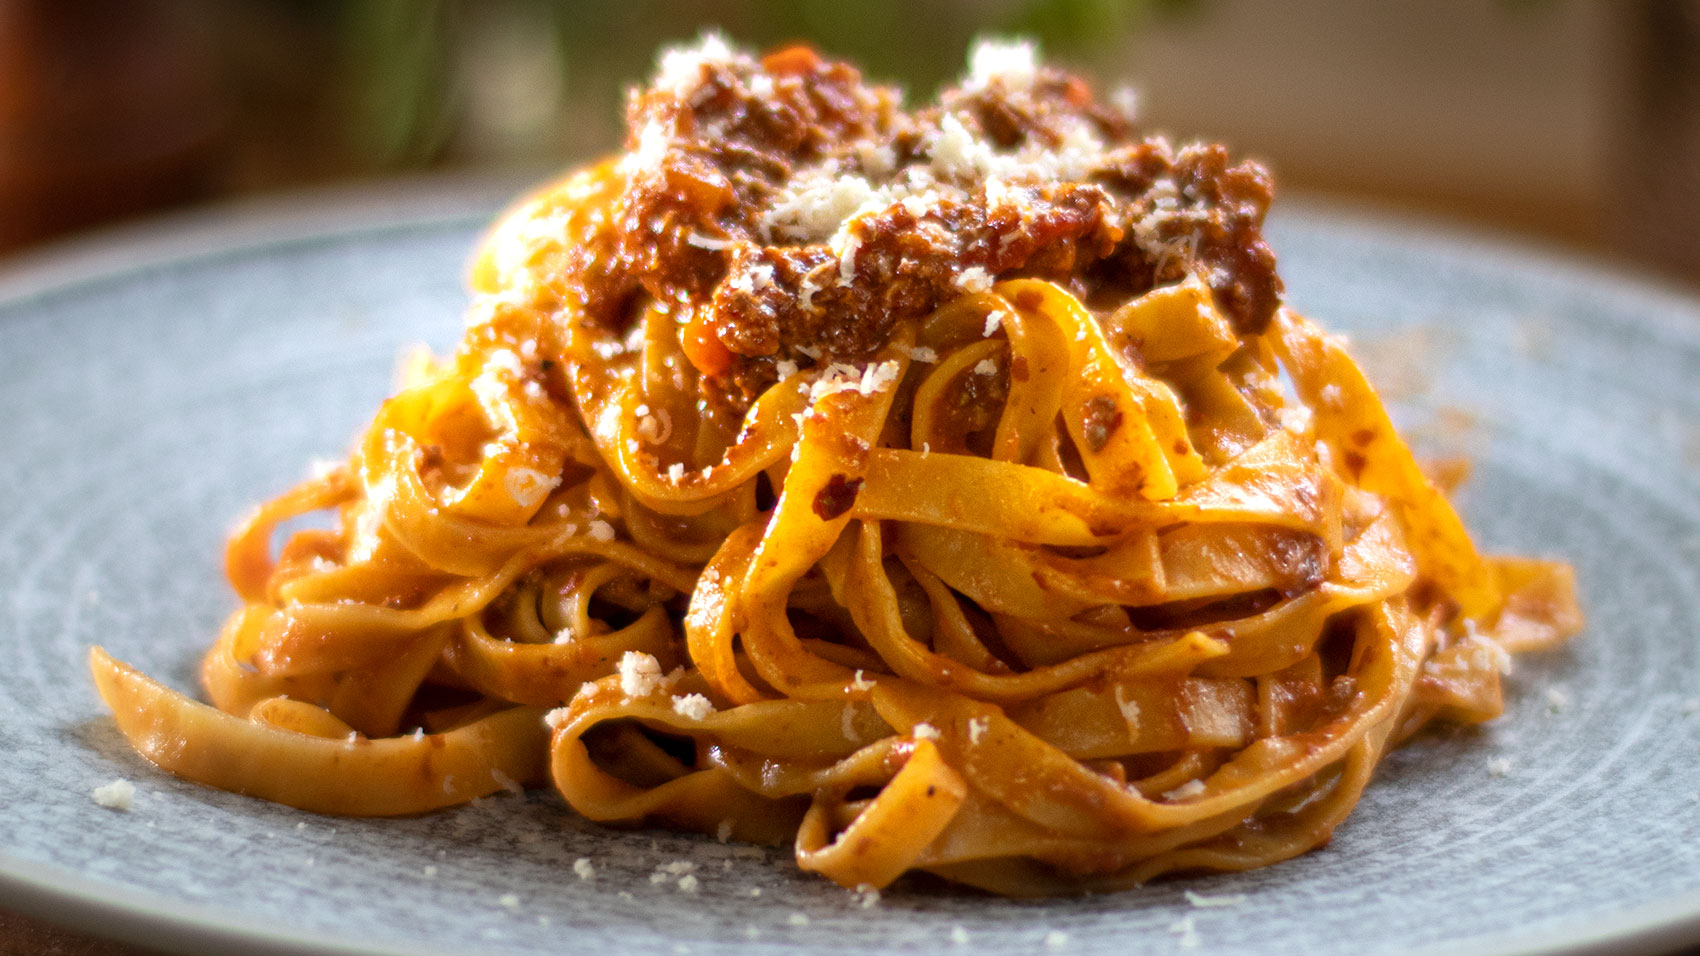
\includegraphics[scale=0.25]{img/page_de_garde.png} \\[1cm]
        \HRule \\[0.4cm]
        { \huge \bfseries LITAL1100/1300 Italien - niveaux élémentaire et moyen \\[0.4cm] }
    
        \HRule \\[1.5cm]
        \textsc{\LARGE Simon Desmidt\\ Issambre L'Hermite Dumont}\\[1cm]
        \vfill
        \vspace{2cm}
        {\large Années académiques 2024-2026}
        \vspace{0.4cm}
         
        
\includegraphics[width=0.15\textwidth]{img/ilv.png}
        
        UCLouvain\\
    
    \end{center}
    \end{sffamily}
\end{titlepage}

\setcounter{tocdepth}{1}
\tableofcontents
\chapter{Conjugaison}
\section{Indicatif présent}
\subsection{Essere/Avere}
\begin{center}
    \begin{tabular}{c|c|c}
        & ESSERE & AVERE \\ \hline
        io & sono & ho\\
        tu & sei & hai\\
        lui/lei/Lei & è & ha\\ 
        noi & siamo & abbiamo \\
        voi & siete & avete \\
        loro & sono & hanno\\
    \end{tabular}
\end{center}
\subsection{Règle générale}
\begin{minipage}{.49\textwidth}
    \vspace{.75cm}
    \begin{center}
        \begin{tabular}{c||c|c|c}
            & ARE & ERE & IRE\\
            \hline
            io & -o & -o & -o\\
            tu & -i & -i & -i\\
            lui/lei/Lei & -a & -e & -e\\
            noi & -iamo & -iamo & -iamo\\
            voi & -ate & -ete & -ite\\
            loro & -ano & -ono & -ono\\
        \end{tabular}
    \end{center}
\end{minipage}
\begin{minipage}{.5\textwidth}
    \centering 
    \begin{figure}[H]
        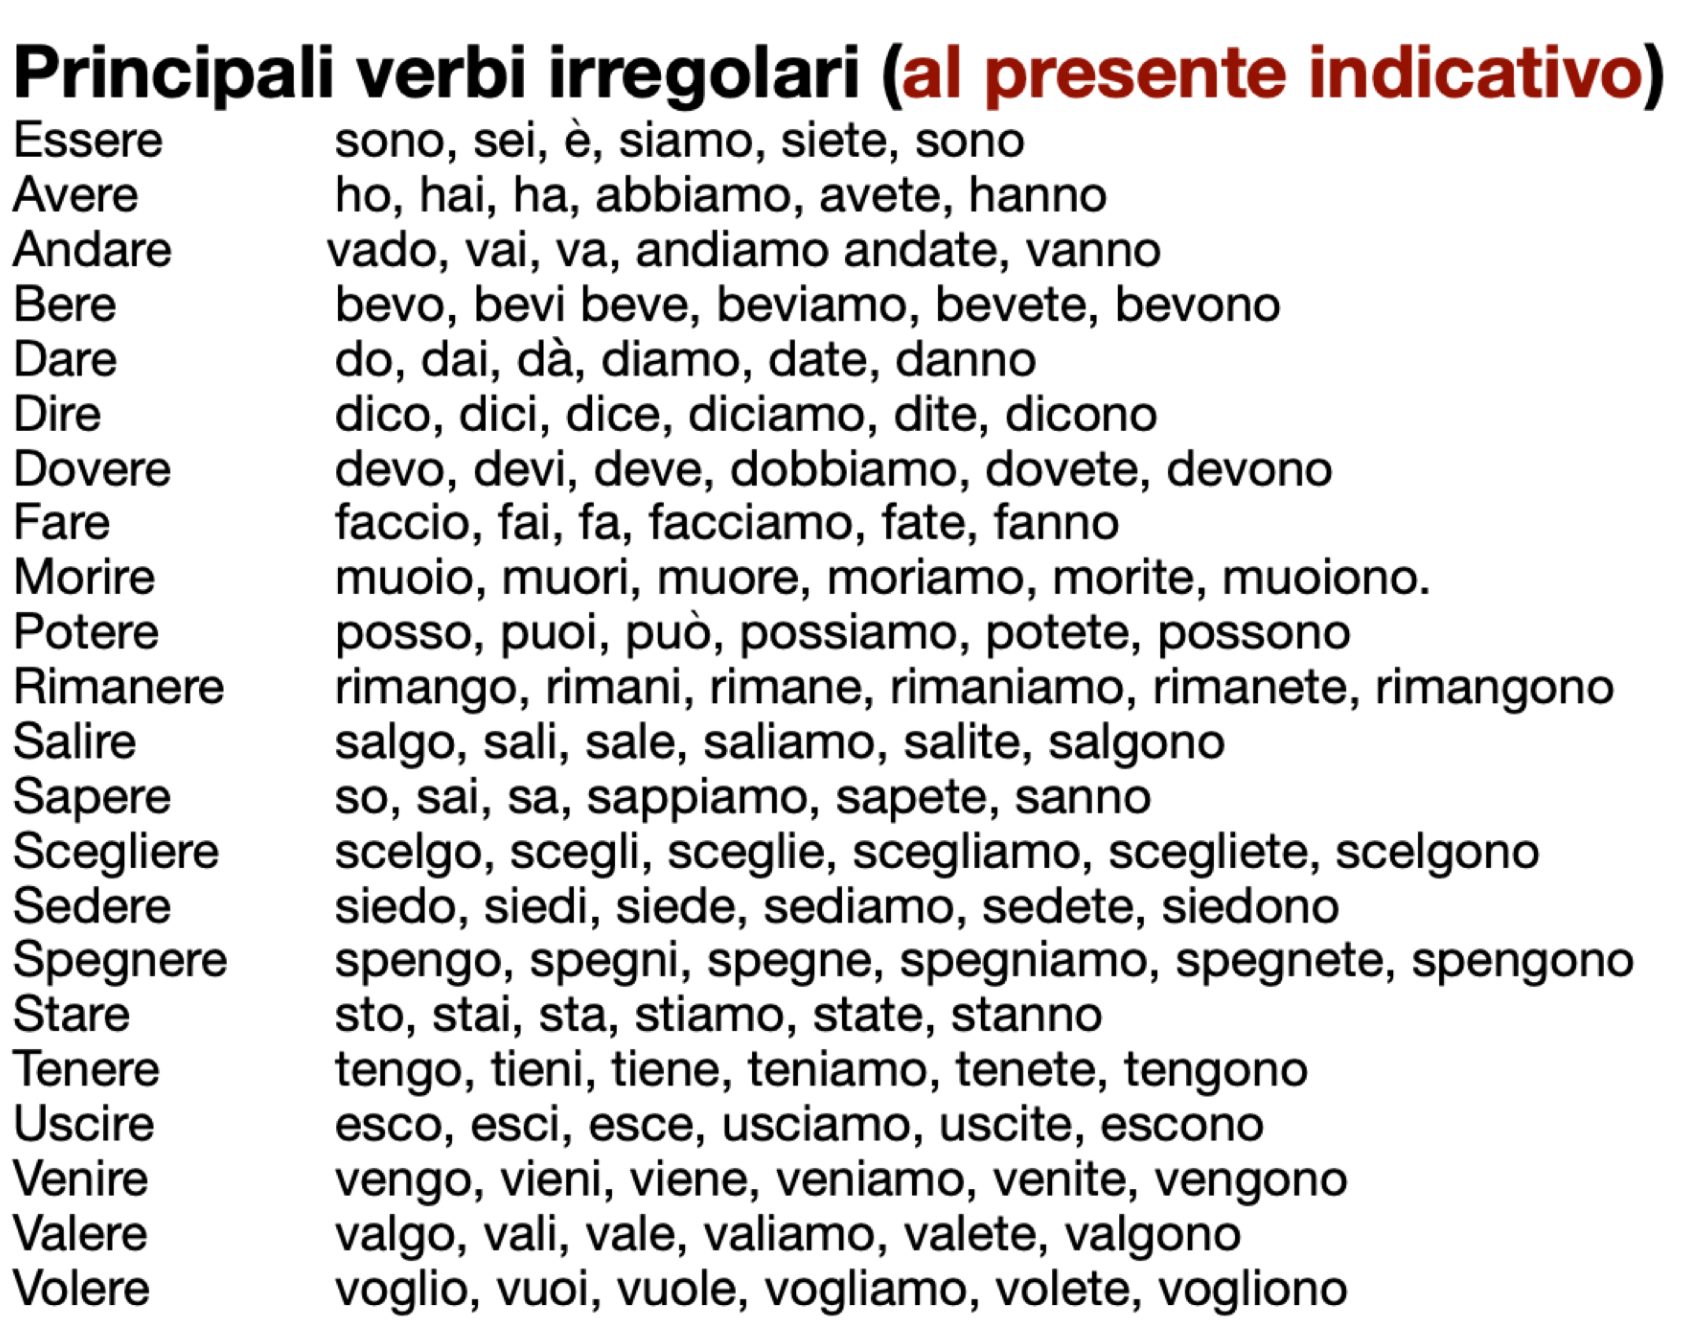
\includegraphics[width = \textwidth]{img/irregolari_presente.png}
    \end{figure}
\end{minipage}\\
\begin{minipage}{.35\textwidth}
    Cas particuliers de spedire (envoyer), preferire (préférer), finire (finir) et capire (comprendre):
    \begin{center}
        \begin{tabular}{c||c}
            io & -isco \\
            tu & -isci \\
            lui & -isce \\
            noi & -iamo \\
            voi & -ite \\
            loro & -iscono \\
        \end{tabular}
    \end{center}
\end{minipage}
\begin{minipage}{.65\textwidth}
    \centering 
    \begin{figure}[H]
        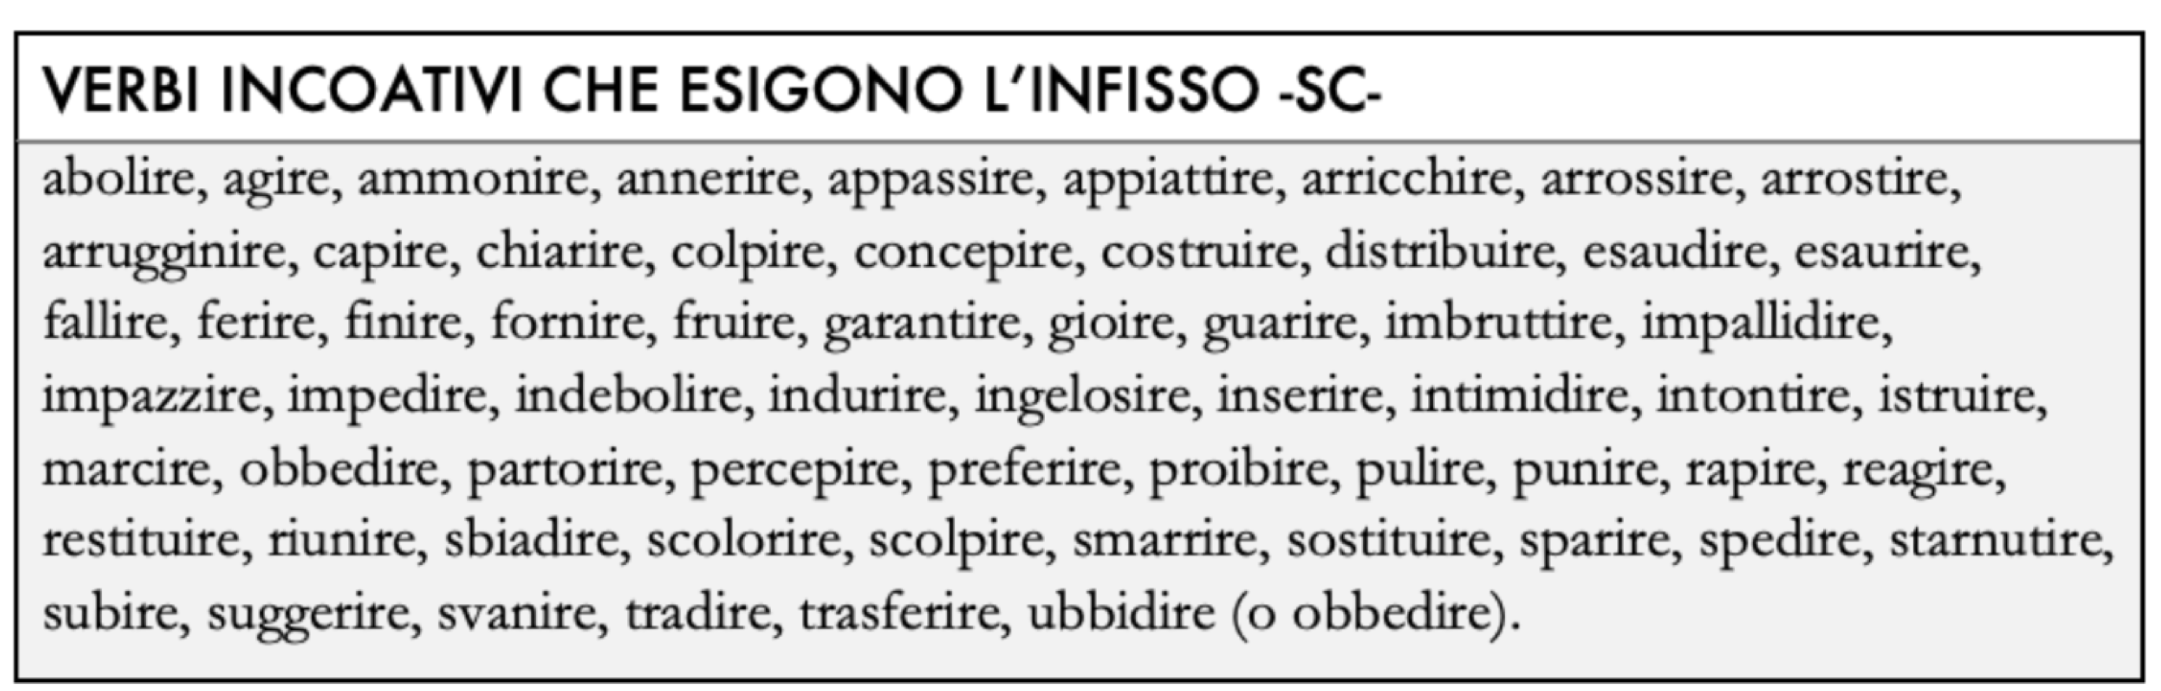
\includegraphics[width = \textwidth]{img/isco.png}
    \end{figure}
\end{minipage}
\subsection{Cas particuliers}
\begin{minipage}{.315\textwidth}
    \begin{center}
        \begin{tabular}{c||c}
            & FARE\\ \hline
            io & faccio\\
            tu & fai\\
            lui & fa\\
            noi & facciamo\\
            voi & fate\\
            loro & fanno\\
        \end{tabular}
    \end{center}
\end{minipage}
\begin{minipage}{.315\textwidth}
    \begin{center}
        \begin{tabular}{c||c}
            & ANDARE\\ \hline
            io & vado\\
            tu & vai\\
            lui & va\\
            noi & andiamo\\
            voi & andate\\
            loro & vanno\\
        \end{tabular}
    \end{center}
\end{minipage}
\begin{minipage}{.315\textwidth}
    \begin{center}
        \begin{tabular}{c||c}
            & VENIRE\\ \hline
            io & vengo\\
            tu & vieni\\
            lui & viene\\
            noi & veniamo\\
            voi & venite\\
            loro & vengono\\
        \end{tabular}
    \end{center}
\end{minipage}
\begin{minipage}{.33\textwidth}
    \begin{center}
        \begin{tabular}{c||c}
            & STARE\\ \hline
            io & sto\\
            tu & stai\\
            lui & sta\\
            noi & stiamo\\
            voi & state\\
            loro & stanno\\
        \end{tabular}
    \end{center}
\end{minipage}
\begin{minipage}{.33\textwidth}
    \begin{center}
        \begin{tabular}{c||c}
            & USCIRE (sortir)\\ \hline
            io & esco\\
            tu & esci\\
            lui & esce\\
            noi & usciamo\\
            voi & uscite\\
            loro & escono\\
        \end{tabular}
    \end{center}
\end{minipage}
\begin{minipage}{.33\textwidth}
    \begin{center}
        \begin{tabular}{c||c}
            & DIRE\\ \hline
            io & dico\\
            tu & dici\\
            lui & dice\\
            noi & diciamo\\
            voi & dicite\\
            loro & dicono\\
        \end{tabular}
    \end{center}
\end{minipage}
\subsection{Verbes réfléchis}
Les verbes réfléchis fonctionnent comme les réguliers, avec les pronoms réfléchis en plus:
\begin{center}
    \begin{tabular}{c||c|c|c|c}
        & & ARE & ERE & IRE\\
        \hline
        io & mi & -o & -o & -o\\
        tu & ti & -i & -i & -i\\
        lui/lei/Lei & si & -a & -e & -e\\
        noi & ci & -iamo & -iamo & -iamo\\
        voi & vi & -ate & -ete & -ite\\
        loro & si &-ano & -ono & -ono\\
    \end{tabular}
\end{center}
\subsection{Volere/Potere/Dovere}
\begin{minipage}{.315\textwidth}
    \begin{center}
        \begin{tabular}{c||c}
            & VOLERE \\ \hline
            io & voglio\\
            tu & vuoi\\
            lui & vuole\\
            noi & vogliamo\\
            voi & volete \\
            loro & vogliono \\
        \end{tabular}
    \end{center}
\end{minipage}
\begin{minipage}{.315\textwidth}
    \begin{center}
        \begin{tabular}{c||c}
            & POTERE \\ \hline
            io & posso \\
            tu & puoi \\
            lui & può\\
            noi & possiamo\\
            voi & potete\\
            loro & possono\\
        \end{tabular}
    \end{center}
\end{minipage}
\begin{minipage}{.315\textwidth}
    \begin{center}
        \begin{tabular}{c||c}
            & DOVERE \\ \hline
            io & devo/debbo\\
            tu & devi \\
            lui & deve \\
            noi & dobbiamo \\
            voi & dovete \\
            loro & devono/debbono\\
        \end{tabular}
    \end{center}
\end{minipage}
\section{Gérondif}
\begin{center}
    \begin{tabular}{c|c|c}
        ARE & ERE & IRE\\ \hline 
        -ando & -endo & -endo\\
    \end{tabular}
\end{center}
Le gérondif sert à former "Stare + gérondif", i.e. "être en train de".
\section{Impératif}
\begin{center}
    \begin{tabular}{c|c|c|c}
        & ARE & ERE & IRE\\ \hline
        tu & -a & -i & -i \\
        noi & -iamo & -iamo & -iamo \\
        voi & -ate & -ete & -ite \\
    \end{tabular}
\end{center}
\begin{itemize}
    \item [$\rightarrow$] Remarque : la seule différence se situe au tu pour les verbes en ARE. 
\end{itemize}
La forme négative est la même pour noi et voi. Elle est "non + infinitif" au tu. 
\subsection{Cas particuliers}
\begin{center}
    \begin{tabular}{c|c}
        vai & va'\\
        fai & fa'\\
        stai & sta'\\
        dai (dare = donner) & da'\\
        dici (dire = dire) & di'\\
        essere & sii/cerca di essere (à l'oral)\\
        avera & abbi\\ 
    \end{tabular}
\end{center}
Quand l'impératif est utilisé avec un pronom (e.g. change-la!), on fusionne le verbe et le pronom, e.g. compraLA, leggiamoLO, apriteLE. 
\section{Imparfait}
\begin{center}
    \begin{tabular}{c|c|c|c}
        & ARE & ERE & IRE\\ \hline
        io & -avo & -evo & -ivo\\
        tu & -avi & -evi & -ivi\\
        lui & -ava & -eva & -iva\\
        noi & -avamo & -evamo & -ivamo\\
        voi & -avate & -evate & -ivate\\
        loro & -avano & -evano & -ivano\\
    \end{tabular}
\end{center}
\begin{itemize}
    \item [$\rightarrow$] Remarque : tous les irréguliers deviennent réguliers, sauf cas très particuliers.
\end{itemize}
\subsection{Cas particuliers}
\begin{minipage}{.315\textwidth}
    \begin{center}
        \begin{tabular}{c||c}
            & ESSERE \\ \hline
            io & ero \\
            tu & eri \\
            lui & era \\
            noi & eravamo \\
            voi & eravate \\
            loro & erano \\
        \end{tabular}
    \end{center}
\end{minipage}
\begin{minipage}{.315\textwidth}
    \begin{center}
        \begin{tabular}{c||c}
            & FARE \\ \hline
            io & facevo \\
            tu & facevi \\
            lui & faceva \\
            noi & facevamo\\
            voi & facevate\\
            loro & facevano \\
        \end{tabular}
    \end{center}
\end{minipage}
\begin{minipage}{.315\textwidth}
    \begin{center}
        \begin{tabular}{c||c}
            & DIRE \\ \hline
            io & dicevo \\
            tu & dicevi \\
            lui & diceva \\
            noi & dicevamo\\
            voi & dicevate \\
            loro & dicevano\\
        \end{tabular}
    \end{center}
\end{minipage}
\section{Forme progressive}
Il existe une forme progressive en conjugaison italienne. Elle se forme comme ceci: 
\begin{center}
    STARE (présent, imparfait, etc) + GERONDIF
\end{center}
Cette forme existe avec tous les temps et sert à décrire des actions en cours, quel que soit le temps  
\section{Passé composé}
Le passé composé se forme comme en français : auxiliaire (essere/avere) + participe passé. On utilise l'auxiliaire avere avec les verbes transitifs, et être avec les autres. 
\subsection{Participe passé}
\begin{center}
    \begin{tabular}{c|c|c}
        ARE & ERE & IRE\\ \hline
        -ato & -uto & -ito\\
    \end{tabular}
\end{center}
Avec l'auxiliaire essere, on fait toujours l'accord entre le sujet et le participe passé. Avec avere, la règle de l'accord est la même qu'en français. 
\begin{itemize}
    \item [$\to$] Remarque : la majorité des verbes -ERE sont irréguliers. 
\end{itemize}
\subsection{Exceptions}
\begin{itemize}
    \item Essere : io sono stato (je suis été et pas j'ai été).
    \item Les verbes qui indiquent le temps utilisent l'auxiliaire essere : il film è durato due ore.
    \item Piacere utilise avere : questo libro mi è piaciuto.
    \item Les verbes de la météo utilisent essere : ieri è piovuto.
\end{itemize}
\section{Plus-que-parfait}
L'utilisation du plus-que-parfait en italien est la même qu'en français. Il se forme avec l'auxiliaire (essere/avere) à l'imparfait + participe passé.
\begin{center}
    ERO / AVEVO + PARTICIPE PASSÉ
\end{center}
\section{Futur simple}
\subsection{Règle générale}
\begin{center}
    \begin{tabular}{c|c|c|c}
        & ARE & ERE & IRE\\ \hline
        io & -erò & -erò & -irò\\
        tu & -erai & -erai & -irai\\
        lui & -erà & -erà & -irà\\
        noi & -eremo & -eremo & -iremo\\
        voi & -erete & -erete & -irete\\
        loro & -eranno & -eranno & -iranno\\
    \end{tabular}
\end{center} 
\subsection{Cas particuliers}
\begin{minipage}{.478\textwidth}
    \begin{center}
        \begin{tabular}{c|c|c}
            Français & Infinitif & Première personne \\ \hline 
            Être & Essere & sarò\\ 
            Avoir & Avere & avrò\\
            Aller & Andare & andrò\\
            Devoir & Dovere & dovrò\\
            Pouvoir & Potere & potrò\\
            Savoir & Sapere & saprò\\
            Voir & Vedere & vedrò\\
            
        \end{tabular}
    \end{center}
\end{minipage}
\begin{minipage}{.478\textwidth}
    \begin{center}
        \begin{tabular}{c|c|c}
            Français & Infinitif & Première personne \\ \hline
            Vivre & Vivere & vivrò\\
            Boire & Bere & berrò\\
            Venir & Venire & verrò\\ 
            Vouloir & Volere & vorrò\\
            Dire & Dire & dirò\\
            Faire & Fare & farò\\
            Être & Stare & starò\\
        \end{tabular}
    \end{center}
\end{minipage}
\begin{itemize}
    \item [$\to$] Remarque : les verbes en -care et -gare ont un h (gherò, cherò).
\end{itemize}
\subsection{Expressions de temporalité}
\begin{center}
    \begin{tabular}{c|c|c|c}
        \multicolumn{2}{c|}{\textbf{Futur}} & \multicolumn{2}{c}{\textbf{Passé}} \\ \hline
        Domani & Demain & Ieri & Hier \\
        Dopodomani & Après-demain & L'altroieri & Avant-hier \\
        Fra/tra due giorni & Dans deux jours & Due giorni fa & Il y a deux jours \\
        La settimana prossima & La semaine prochaine & La settimana scorsa & La semaine passée \\
        Domani mattina & Demain matin & Ieri mattina & Hier matin \\
        Domani sera/notte & Demain soir & Ieri sera & Hier soir \\
    \end{tabular}
\end{center}
\section{Futur antérieur}
\begin{center}
    Essere/Avere (futur simple) + Participe passé 
\end{center}
\begin{itemize}
    \item [$\to$] Remarque : l'utilisation est la même qu'en français.
\end{itemize}
\section{Random}
\begin{center}
    Avere + appena + fatto + infinitif 
\end{center}
Cette formulation signifie "venir de faire", et avere peut se conjuguer à tous les temps.
\section{Conditionnel présent}
\begin{center}
    \begin{tabular}{c|c|c|c}
        & ARE & ERE & IRE\\ \hline
        io & -erei & -erei & -irei\\
        tu & -eresti & -eresti & -iresti\\
        lui & -erebbe & -erebbe & -irebbe\\
        noi & -eremmo & -eremmo & -iremmo\\
        voi & -ereste & -ereste & -ireste\\
        loro & -erebbero & -erebbero & -irebbero\\
    \end{tabular}
\end{center} 
Son utilisation est la même qu'en français. 
\subsection{Irréguliers}
\begin{center}
    \begin{tabular}{c|c||c|c||c|c}
        Infinitif & Forme irrégulière & Infinitif & Forme irrégulière & Infinitif & Forme irrégulière\\ \hline 
        Essere & sarei & Avere & avrei & Bere & berrei\\
        Dare & darei & Andare & andrei & Rimanere & rimarrei\\
        Dire & direi & Dovere & dovrei & Venire & verrei\\
        Fare & farei & Potere & potrei & Volere & vorrei\\
        Stare & starei & Sapere & saprei & Tenere & terrei\\
        Avere & avrei & Vedere & vedrei & Tradurre & tradurrei\\
    \end{tabular}
\end{center}
\section{Conditionnel passé}
\begin{center}
    Avere/Essere (Conditionnel présent) + participe passé
\end{center}
Son utilisation est la même qu'en français. 
\section{Participes passés irréguliers}
\begin{minipage}{.5\textwidth}
    \begin{center}
        \begin{tabular}{c|c|c}
            Infinitif & Participe passé & Traduction\\ \hline 
            Accendere & acceso & allumer \\
            Chiudere & chiuso & fermer \\
            Mettere & messo & mettre \\
            prendere & preso & prendre \\
            Rispondere & risposto & répondre \\
            Spendere & speso & dépenser \\
            Chiedere & chiesto & demander\\
            Leggere & letto & lire \\
            Perdere & perso/perduto & perdre \\
            Rimanere & rimasto & rester \\
            Scrivere & scritto & écrire \\
            Vedere & visto & voir \\
            Fare & fatto & faire\\
            Aprire & aperto & ouvrir\\
            Venire & venuto & venir\\
            Dire & detto & dire\\
            Offrire & offerto & offrir\\
            Bere & bevuto & Boire\\
            Correggere & corretto & corriger\\
            Decidere & deciso & décider\\
            Dividere & diviso & diviser\\
            Muovere & mosso & bouger\\
        \end{tabular}
    \end{center}
\end{minipage}
\begin{minipage}{.5\textwidth}
    \begin{center}
        \begin{tabular}{c|c|c}
            Infinitif & Participe passé & Traduction\\ \hline
            Nascondere & nascosto & cacher\\
            Piangere & pianto & pleurer\\
            Proporre & proposto & proposer\\
            Rompere & rotto & casser\\
            Convincere & convinto & convaincre\\
            Correre & corso & courir\\
            Discutere & discusso & discuter\\
            Friggere & fritto & frire\\
            Nascere & nato & naître\\
            Offendere & offeso & offenser\\
            Promettere & promesso & promettre\\
            Ridere & riso & rire\\
            Scegliere & scelto & choisir\\
            Vivere & vissuto & vivre\\
            Vincere & vinto & vaincre\\
            Tradurre & tradotto & traduire\\
            Succedere & successo & arriver\\
            Spingere & spinto & pousser\\
            Sorprendere & sorpreso & surprendre\\
            Smettere & smesso & arrêter\\
            Scendere & sceso & descendre\\
            Il en manque &un pour avoir &de belles lignes\\
        \end{tabular}
    \end{center}
\end{minipage}
\chapter{Grammaire}
\section{Accents}
Il existe des catégories de mots selon l'accent tonique:
\begin{itemize}
    \item tronche : accent sur la dernière syllabe (virtù, perché, caffè, città,...)\footnote{Les accents s'écrivent toujours sur la dernière syllabe.};
    \item piane : accent sur l'avant-dernière syllabe (sapòne, tènda, mangiàre, capìto,...)\footnote{Ici et pour les catégories suivantes, l'accent n'est écrit que pour illustrer, le mot réel ne le contient pas.};
    \item sdrucciole : accent sur l'antépénultième syllabe (tàvolo, mènsile, gòndola,...);
    \item bisdrucciole : accent sur la quatrième syllabe en partant de la fin (telèfonami, dìtelemo,...);
    \item trisdruciole : accent sur la cinquième syllabe en partant de la fin (rècitamelo,...).
\end{itemize}
\section{Terminaisons des noms et adjectifs}
\begin{center}
    \begin{tabular}{c|c|c}
        Singulier & Pluriel & Cas\\
        \hline
        -o & -i & Masculin \\
        -a & -e & Féminin \\
        -e & -i & Masculin ou féminin\\
    \end{tabular}
\end{center}
\begin{itemize}
    \item [$\rightarrow$] Remarque : Si un -cia ou un -gia est précédé d'une consonne, le i tombe au pluriel (-ce, -ge).
\end{itemize}
L'adjectif vient en général après le nom.
\subsection{Irréguliers}
\begin{center}
    \begin{tabular}{c|c|c}
        Singulier & Pluriel & Traduction\\ \hline 
        L'orecchio & Le orecchie & l'oreille \\
        Il braccio & Le braccia & le coeur \\
        Il ginocchio & le ginocchia & le genou\\
        Il dito & le dita & le doigt\\
        Il centinaio & le centinaia & la centaine \\
        Il migliaio & le migliaia & le millier \\
        Il paio & le paia & le couple \\
        L'uovo & le uova & l'oeuf \\
        L'uomo & gli uomini & l'homme\\
        Il bue & i buoi & le boeuf\\
        Il tempio & i templi & le temple \\
        Il dio & gli dei & le dieu\\
        L'ala & le ali &l'aile \\
        la mano & le mani & la main\\
        l'arma & le armi & l'arme\\
    \end{tabular}
\end{center}
\section{Déterminants}
\begin{center}
    \begin{tabular}{c|c|c|c|c}
        \multicolumn{2}{c|}{Déterminés} & \multicolumn{2}{c|}{Indéterminés} & \\ \hline
        Singulier & Pluriel & Singulier & Pluriel & \\
        La & Le & Una & Delle & Féminin commençant par une consonne \\ 
        L' & Le & Un' & Delle & Féminin commençant par une voyelle \\ 
        Lo & Gli & Uno & Degli & Masculin commençant par s+consonne, xyz, psi, etc\\ 
        L' & Gli & Un & Degli & Masculin commençant par une voyelle \\ 
        Il & I & Un & Dei & Masculin \\ 
    \end{tabular}    
\end{center}
\section{Prépositions}
\subsection{Prépositions utilisées avec l'article}
\begin{figure}[H]
    \centering
    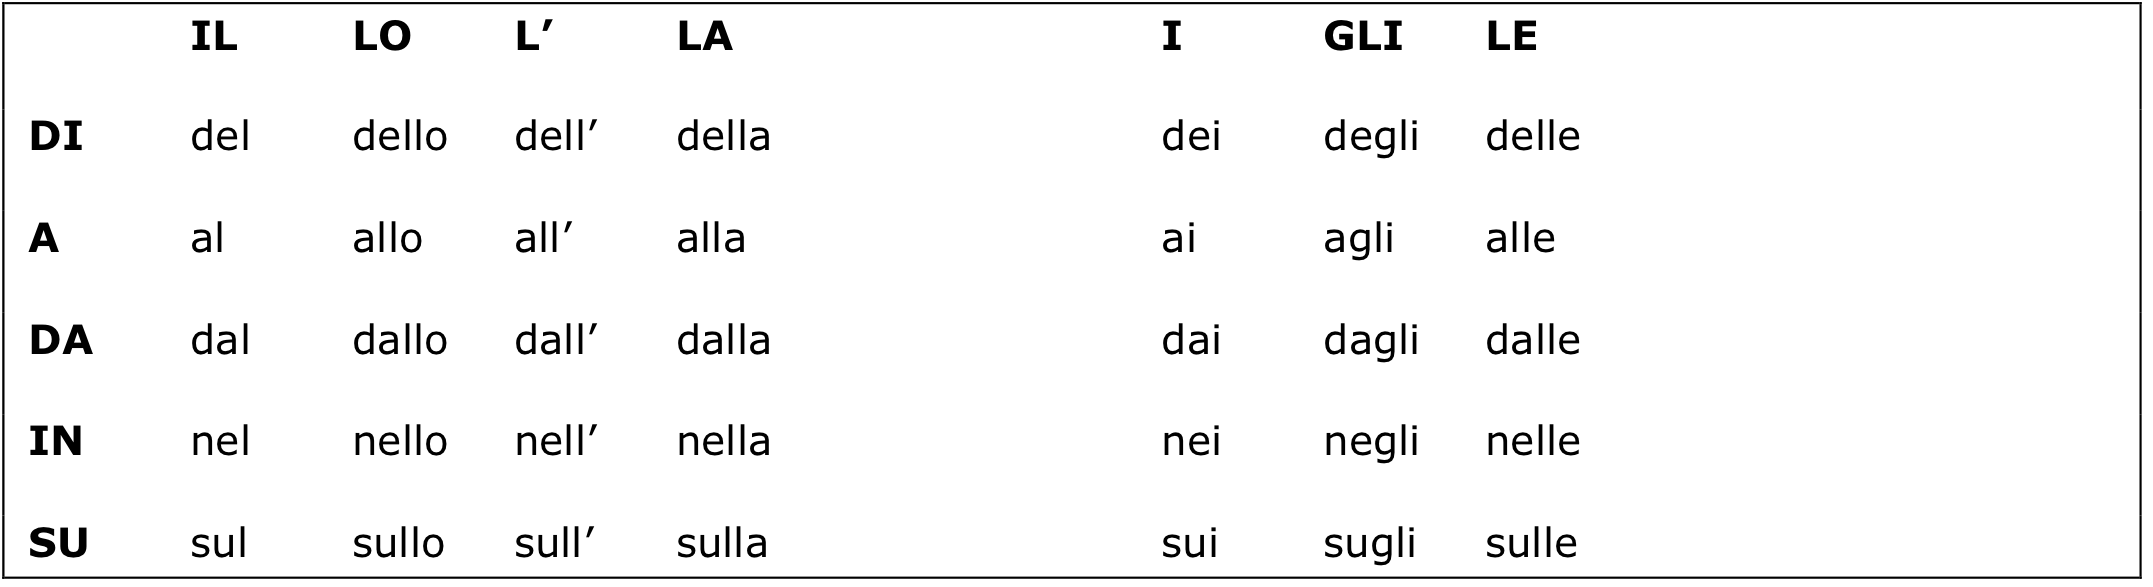
\includegraphics[width = \textwidth]{img/prep.png}
\end{figure}
Les prépositions con, per, tra, fra sont utilisées avec article séparé. 
\section{Adjectifs et pronoms possessifs}
\begin{center}
    \begin{tabular}{c|c}
        Pronom & Correspondance\\ \hline
        il mio/ il tuo/ il suo/ il nostro/ il vostro/ il loro & uno \\
        la mia/ la tua/ la sua/ la nostra/ la vostra/ la loro & una\\
        i miei/ i tuoi/ i suoi/ i nostri/ i vostri/ i loro & i\\
        le mie/ le tue/ le sue/ le nostre/ le vostre/ le loro & le\\
    \end{tabular}
\end{center}
\begin{itemize}
    \item [$\rightarrow$] On ne met pas l'article s'il s'agit d'un membre de la famille au singulier, SAUF pour loro et si le nom est modifié par un adjectif diminiutif/"augmentant", e.g. la mia cara sorella, il mio fratellino.
\end{itemize}
\section{Pronoms}
\begin{center}
    \begin{tabular}{c|c|c|c|c|c}
        Pronom sujet & \multicolumn{2}{c|}{Pronom direct} & \multicolumn{2}{c|}{Pronom indirect} & Pronom réfléchi \\ \hline 
        & Faible & Fort & Faible & Fort & \\ \hline 
        io & mi & me & mi & a me & mi\\
        tu & ti & te & ti & a te & ti\\
        lui/lei/Lei & lo/la/La & lui/lei/Lei & gli/le/Le & a lui/a lei/a Lei & si/Si\\
        noi & ci & noi & ci & a noi & ci\\
        voi & vi & voi & vi & a voi & vi\\
        loro & li/le & loro & gli & a loro & si\\
    \end{tabular}
\end{center}
\begin{itemize}
    \item [$\to$] Remarque : Lorsque lo/la suit un auxiliaire, il devient l'apostrophe l' (e.g. l'ho visto). Cela n'est pas vrai avec les pronoms du pluriel.
    \item [$\to$] Remarque : la forme forte est utilisée pour insister sur le pronom.
\end{itemize}
\chapter{Divers}
\underline{Fichiers :}
\begin{itemize}
    \item \texttt{preposizioni riassunto}
    \item \texttt{Espressioni con Essere Fare Avere}
    \item Molto, troppo, poco s'accordent avec le nom quand ils sont adjectifs. 
\end{itemize}
\section{Heure}
\begin{center}
    \begin{tabular}{c|c}
        è mezzogiorno  & il est midi\\
        è mezzanotte & il est minuit\\
        è l'una & il est 1h\\
        sono le X & il est Xh (X>1)\\
        sono le X meno Y & il est Xh moins Y.\\
        sono le X e Y & il est XhY.\\
        sono le X e mezza/o & il est Xh30.\\
        sono le X e un quarto & il est Xh15.\\
        sono le X di mattina & il est Xh du matin.\\
        sono le X di sera & il est Xh du soir.\\
        sono le X in punto & il est Xh pile.\\
    \end{tabular}
\end{center}
\section{Vocabulaire}
Le lien Quizlet pour le vocabulaire de LITAL 1100 est \hyperlink{https://quizlet.com/be/1006471421/lital1100-q2-flash-cards/}{ici}.
\end{document}